\documentclass[11pt]{article}
\usepackage[spanish]{babel}
\usepackage[utf8]{inputenc}
\usepackage[T1]{fontenc}
\usepackage{graphicx}
\topmargin=-1.2cm
\textheight=22cm
\textwidth=16cm  
\oddsidemargin=0.45cm  
\setlength{\parindent}{0cm}
\renewcommand{\baselinestretch}{1.1}
\graphicspath{{hola/}}
\title{Actividad 6}
\author{Hinostroza Moya Natalia}
\date{05 de abril de 2017}

\begin{document}
%===============================================================================
% PORTADA
%===============================================================================
\begin{titlepage}
\begin{center}
\includegraphics[scale=0.35]{escudo.png}
\end{center}
\vspace*{0.02in}
\begin{center}

\rmfamily\textbf{\LARGE UNIVERSIDAD DE SONORA}\\
\vspace*{1.02in}
{\Large División de Ciencias Exactas y Naturales}\\
{\Large Departamento de Física}\\

\vspace*{0.99in}
\rule{99mm}{0.1mm}\\
\vspace*{0.4cm}
\textbf{\LARGE Análisis Armónico de Mareas}\\
\vspace*{0.001in}
\rule{99mm}{0.1mm}

\vspace*{1in}
\normalsize{Autor:}\
\normalsize{Natalia Hinostroza Moya}\\
\vspace*{0.3mm}
\normalsize Profesor:\
\normalsize Carlos Lizárraga Celaya\\
\vspace*{1.5cm}
\normalsize 05 de abril de 2017

\end{center}
\end{titlepage}

%==============================================================================
% DESARROLLO
%==============================================================================
\textbf{\section*{\LARGE Resumen}}
En esta actividad se encuentran las gráficas de los analisis armónicos de los datos obtenidos anteriormente en sondeos de mareas. En ella se encuentran los nombres de cada uno de los componentes principales de las mareas.

\textbf{\section{\LARGE Introducción}}
Para llevar a cabo esta actividad se analizaron los datos ya obtenidos anteriormente de los lugares seleccionados, en este caso Mazatlán y San Francisco. Con la ayuda de fftpack, obtuvimos las principales componentes de Fourier de las mareas de cada sitio y se graficaron. Con la ayuda de la tabla que se encuentra en el artículo de \underline{Teoría de Mareas} de la Wikipedia, reconocimos el nombre y origen de cada una de las mareas.

\textbf{\section{\LARGE Análisis de Fourier}}
El análisis de Fourier o análisis armónico, en matemáticas estudia la representación de funciones o señales como superposición de ondas "básicas" o armónicas.\\

Una de las ramas más modernas del análisis armónico, que tiene sus raíces a mediados del siglo XX, es el análisis sobre grupos topológicos. El ideal central que lo motiva es la de las varias transformadas de Fourier, que pueden ser generalizadas a una transformación de funciones definidas sobre grupos localmente compactos.

\textbf{\section{\LARGE Graficas del Análisis Armónico de Mareas}}

\textbf{\subsection{\Large Mazatlán, Sinaloa.}}

Elcódigo utilizado para realizar la gráfica que se presenta a continuación fue el siguiente:\\ 

\begin{verbatim}
N = 720
T =  1
y = df['altura(mm)']
yf = fft(y)
xf = fftfreq(N, T)
xf = fftshift(xf)
yplot = fftshift(yf)
import matplotlib.pyplot as plt
plt.plot(xf, 1.0/N * np.abs(yplot))
plt.xlim(0,0.10)
plt.title('Mazatlán, Sinaloa.')
plt.xlabel('Frecuencia')
plt.ylabel('Nivel del Mar')

plt.grid()
fig=plt.gcf()
fig.set_size_inches(7,7)
plt.show()

\end{verbatim}

En donde pedimos que se grafique la frecuencia con respecto a la altura con ayuda fftpack. En N indicamos el número de muestras con las que contamos y en T el periodo.\\

\begin{center}
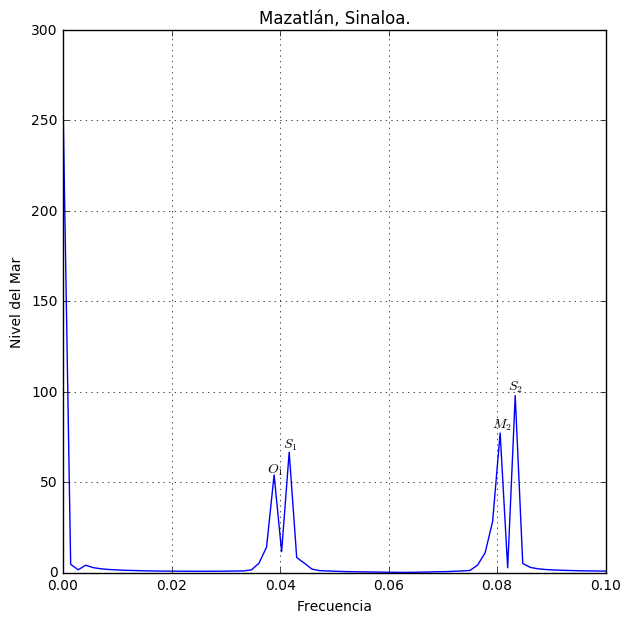
\includegraphics[scale=0.70]{Mazatlan6.png}
\end{center}

Con la frecuencia calculamos el valor aproximado del periodo para poder etiquetar las componentes de las mareas con la infromación de la tabla de Teoria de Mareas.\\

Para poner los nombres en la gráfica utilizamos el siguiente código:\\

\begin{verbatim}
plt.text(.0375,55,"$O_1$")
plt.text(.04055,69,"$S_1$")
plt.text(.079,80,"$M_2$")
plt.text(.082,101,"$S_2$")
\end{verbatim}

En donde indicamos la coordenada y el nombre que uqeremos poner. 

\textbf{\subsection{\Large San Francisco, CA.}}
Para la siguiente gráfica se utilizó el mismo procedimiento que en la anterior.\\ 

El código es:\\

\begin{verbatim}
N = 720
T =  1
y = df['Water Level']
yf = fft(y)
xf = fftfreq(N, T)
xf = fftshift(xf)
yplot = fftshift(yf)
import matplotlib.pyplot as plt
plt.plot(xf, 1.0/N * np.abs(yplot))
plt.xlim(0,0.1)
plt.title('San Francisco, CA')
plt.xlabel('Frecuencia')
plt.ylabel('Nivel del Mar')
plt.grid()
fig=plt.gcf()
fig.set_size_inches(7,7)

plt.text(.0375,0.11,"$O_1$")
plt.text(.0406,0.15,"$K_1$")
plt.text(.079,0.3,"$M_2$")
plt.text(.0825,0.093,"$S_2$")

plt.show()
\end{verbatim}

\begin{center}
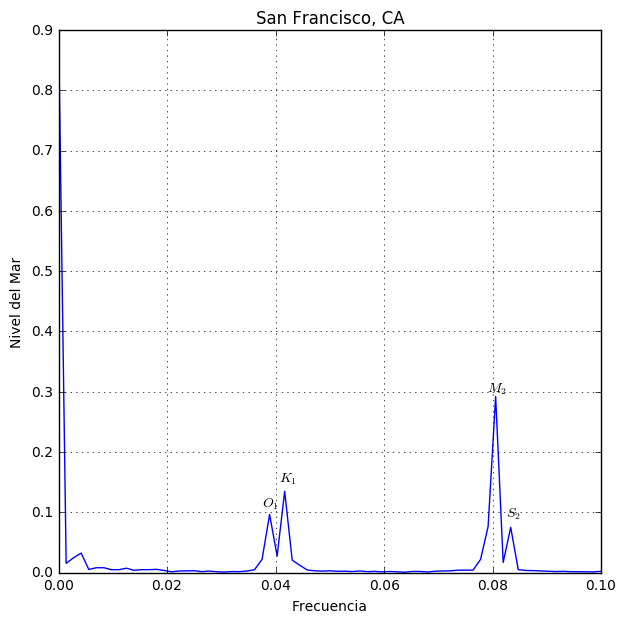
\includegraphics[scale=0.70]{SF6.png}
\end{center}

\textbf{\section{\LARGE Principales Componentes Armónicos de las Mareas}}
% TABLA 
\begin{table}[htbp]
\begin{center}
\begin{tabular}{|l|l|l|}
\hline \hline
Nombre & Símbolo & Periodo (hrs)  \\
\hline \hline
Límite de agua superficial de la luna principal & $M_{4}$ & 6.210300601 \\ \hline
Límite de agua superficial de la luna principal & $M_{6}$ & 4.140200401 	\\ \hline
Agua superficial terdiurnal & $MK_{3}$ & 8.177140247 \\ \hline
Abundancia de agua poco profunda de la energía solar principal & $S_{3}$ & 6 \\ \hline
Cuarto de agua poco profunda diurna &  $MN_{4}$  & 6.269173724 \\ \hline
Principal lunar semidiurno & $M_{2}$ & 12.4206012 \\ \hline
Principal solar semidiurno & $S_{2}$ & 12 \\ \hline
Gran lunar elíptica semidiurna & $N_{2}$ & 12.65834751 \\ \hline
Lunar diurno & $K_{1}$ & 23.93447213  \\ \hline
Lunar diurno & $O_{1}$ & 25.81933871 \\ \hline
\end{tabular}
\label{tabla:sencilla}
\end{center}
\end{table}

\end{document}

